\documentclass{article}
\usepackage{titlesec}
\usepackage{mhchem}
\usepackage{array}
\usepackage{graphicx}
\usepackage[bmargin=2cm, tmargin=2cm]{geometry}
\usepackage{fourier-orns}
\usepackage{chemfig}
\usepackage{subfig}
\usepackage{amsmath}
\newcommand{\A}{\text{\normalfont\AA}}


\renewcommand{\sup}[1]{\(^#1\)}
\newcommand{\sub}[1]{\(_#1\)}
\newcommand{\thedate}[1]{\hfill{\small\sc #1}}
\newcommand{\NB}{{\large\lefthand}\quad}
\renewcommand{\deg}{\text{\(^\circ\)}}
\titleformat{\section}[hang]{\sc\Large}{\S\thesection}{3ex}{}[]
\titleformat{\subsection}[runin]{\sc\large}{\S\thesubsection}{3ex}{}[]
\titleformat{\subsubsection}[runin]{}{\S\thesubsubsection}{1ex}{\bfseries}[.]

\newtheorem{defn}{Definition}[section]

\title{Intermediate Inorganic Chemistry}
\date{}
\begin{document}
    \maketitle
    \section{P-block Chemistry}
    \subsection{Metalloids}
    \subsection{Electronegativity}\thedate{28/10/20 --- Week 1}
    \subsubsection{Ionisation Energy (IE)} The energy required to remove completely
    an electrion from the gaseous atom or molecule in its `ground state'.

    \begin{center}
        {\renewcommand{\arraystretch}{2}%
        \begin{tabular}[2cm]{l l}
            \ce{ M_{(g)} -> M^+_{(g)} + e-}  & First Inonisation Energy \\
            \ce{M^2+_{(g)} -> M^3+_{(g)} + e-} & Second Inonisation Energy
        \end{tabular}}
    \end{center}
        
    This process requries an input of energy (endothermic), 
    so the ionisation energy will be positive.

    Concerning the p (and s) blocks the inionisation energy increases from
    left to right (with some exceptions) and sharply decreases upon a new period. The higher (in number) the
    period the lower the ionisation energy.
    The most important factor is the distance between the nucleus and electron. With larger shells (e.g. p) the electrons
    are further away and so are not pulled on as heavily by the nucleus (lower effective nuclear charge).
    Notice on the graph where the ionisation energy does not increase across the period.
    
    \begin{figure}[h]
        \centering
        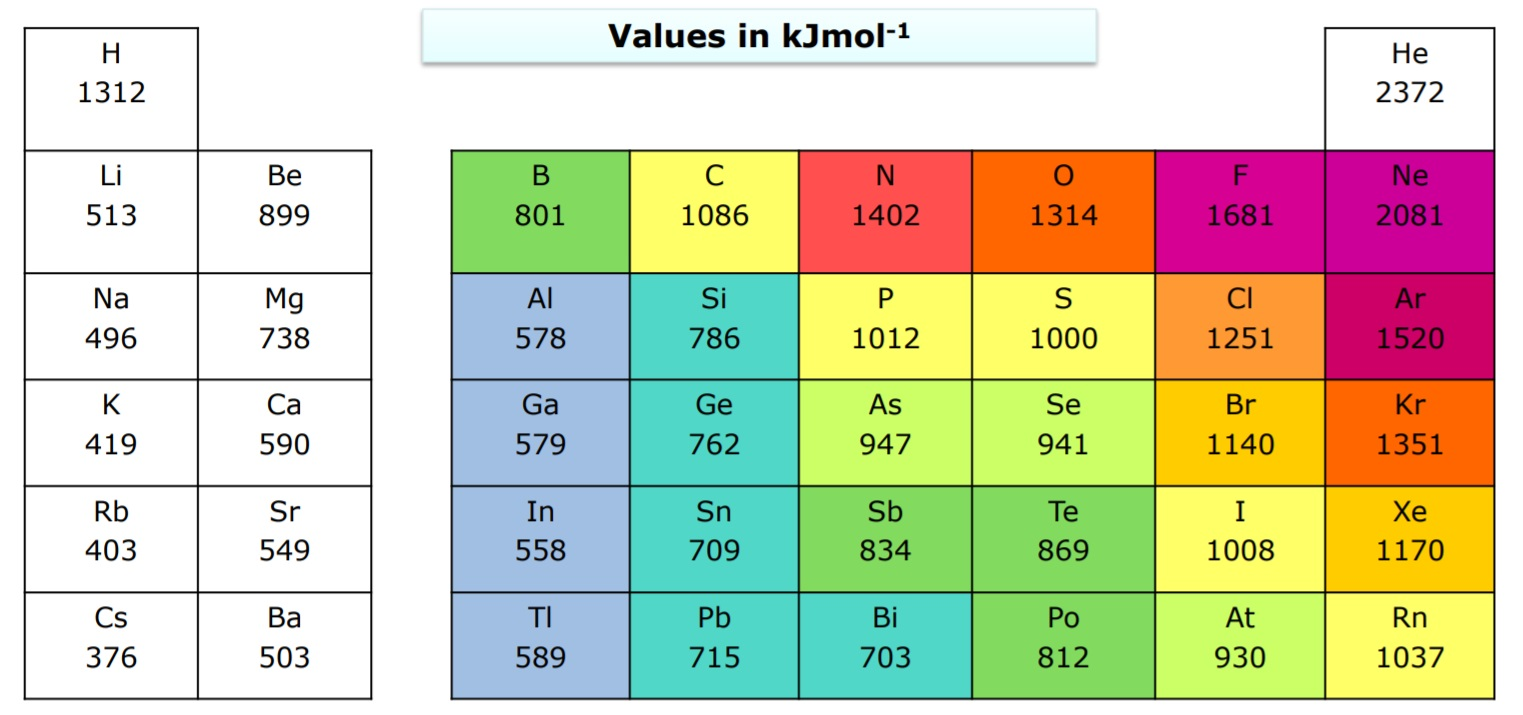
\includegraphics[width=12cm]{ionisation energy.jpg}
    \end{figure}
    \NB The ionisation energy of the metalloids are very similar (801--812), the increase in energy of going across the period
    is counteracted by moving down the table. 

    On descending groups the most irregular behaviour is seen in group 13. Ga and Ti are \emph{higher} than
    expected. Ga is preceded by the first set of d orbitals and Ti is preceded by the first set of f orbitals.
    d and f orbitals provide very weak shielding in comparison to s and p orbitals, so we have a higher effective
    nuclear charge than expected.
    Pb breaks the trend down its group, this is because the atom is much larger than the others in its group, and
    so its electrons are moving much faster, these relativistic effects make it much harder to remove an electron.

    \begin{figure}[h]
        \centering
        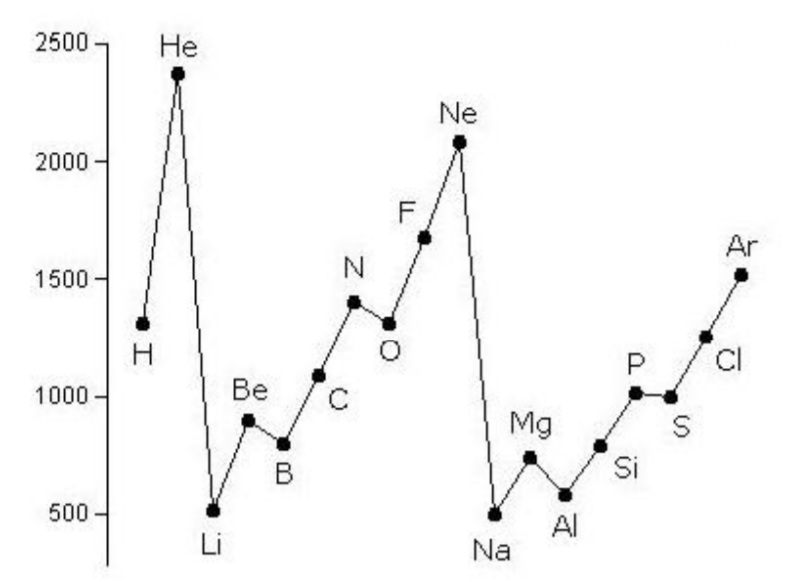
\includegraphics[width=6cm]{group13.jpg}
    \end{figure}

    The kink from Be to B comes from the Be having a full s shell, so removing an electron from Boron would be 
    favourable to give it a full s-orbital. The kink from N to O comes from Oxygen having a paired electron in its
    p-orbital, so they experience greater \emph{Coulombic repulsion}. The removal of an electron relieves this
    repulsion.

    \subsubsection{Electron Affinity (EA)} The energy release when a gaseous atom,
    molecule or ion in its `ground state' gains an electron.
    \begin{center}
        \ce{X_{(g)} + e- -> X^-_{(g)}} \hspace{4ex} First electron Affinity
    \end{center}

    Since this process is favourable and energy will be given out (exothermic),
    this electron affinity will be negative.

    \begin{figure}[h]
        \centering
        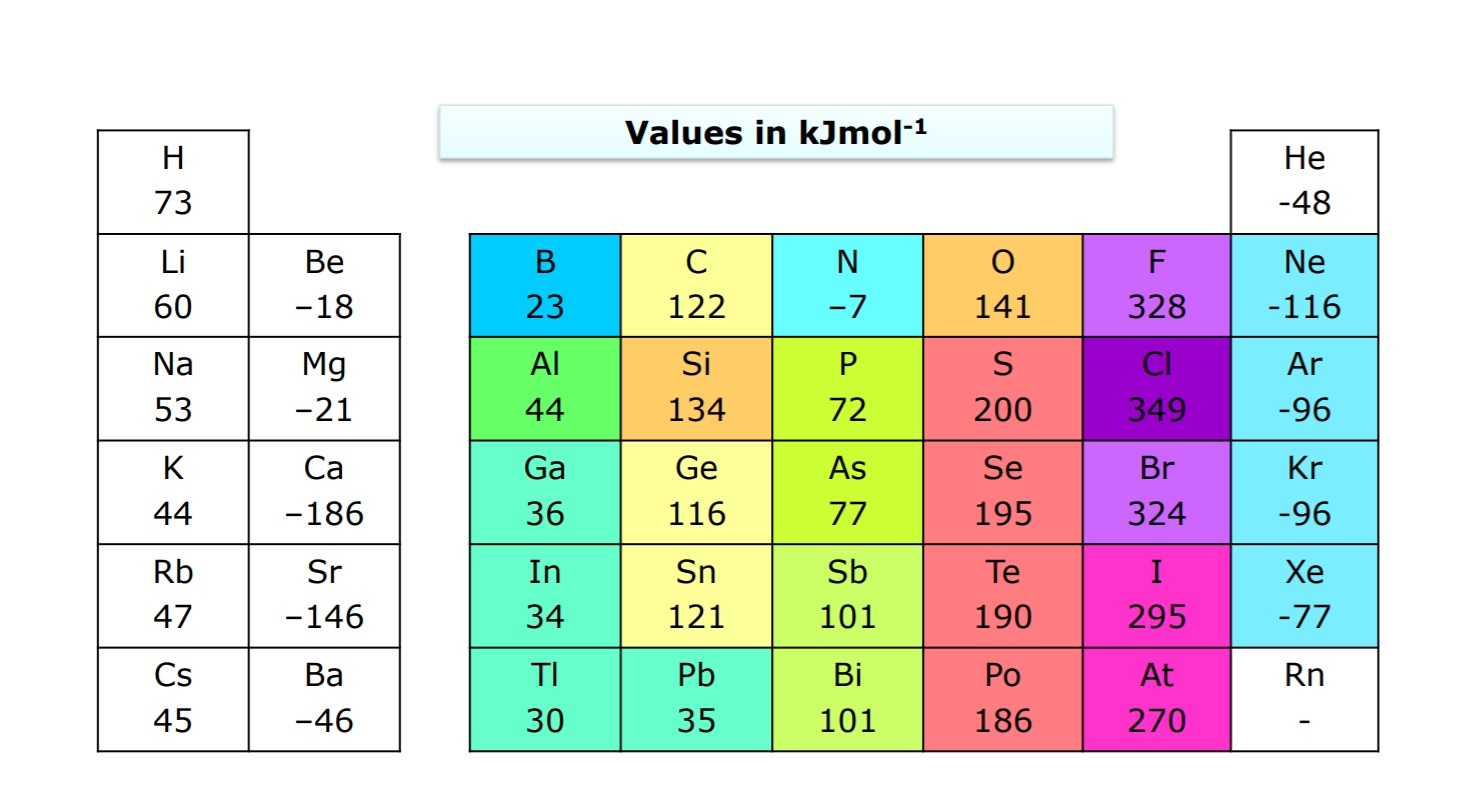
\includegraphics[width=12cm]{ea.jpg}
    \end{figure}
    \NB A positive value corresponds to energy being given out upon addition of an electron. Negative enthalpy.

    It is very unfavourable for Neon to accept an electron and break its full p orbital, and very favourable for
    Fluorine to accept an electron and fufill its shell. It generally gets smaller as you move down a group
    due to more shielding. Nitrogen's value is negative because of the energy needed to overcome the electron-
    electron repulsion that occurs when two electrons occupy the same orbital (think back to IE). 
    The same applies to all of group 15. Group 2 is also lower because it already has a full shell.
    The values of Group 13 (except for B) are all very similar due to the weak shielding provided by the 
    preceding d and f orbitals.
    The 2nd period is is smaller than the first becuase of the small size, so it has a higher charge to radius 
    ratio which gives higher repulsion.
    \begin{figure}[h]
        \centering
        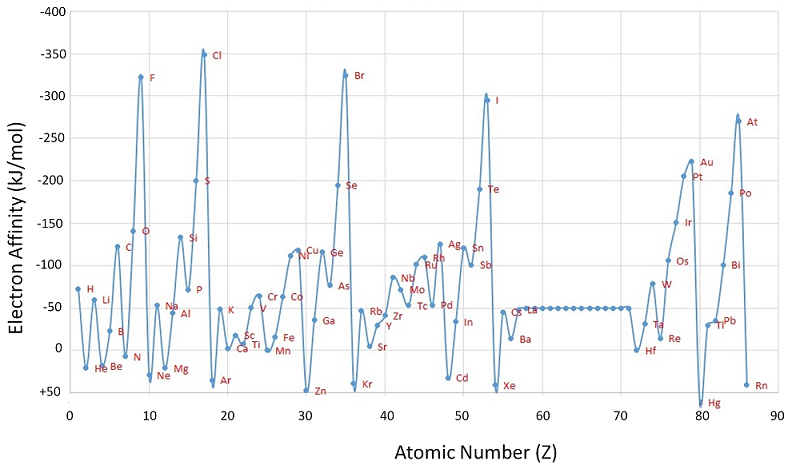
\includegraphics[width=12cm]{ea2.png}
    \end{figure}
    \newpage
    \subsubsection{Electronegativity} The ability of an atom to attract electron density towards itself in a molecule.
    
    The calculation of electronegativity using the Pauling scale.
    \begin{enumerate}
        \item A hypothetical molecule XY
        \item Compare the measured \(XY_{\text{measured}}\) bond energy with a theoretical bond energy \(XY_{\text{theoretical}}.\)
        \item \(XY_{\text{theoretical}} = \sqrt{XX^2 + YY^2}\)
        \item \(\Delta\) Bond energy = \(XY_{\text{measured}} - XY_{\text{theoretical}}\)
    \end{enumerate}

    A difference in bond energy implies a difference in electronegativity between the two atoms.
    \begin{figure}[h]
        \centering
        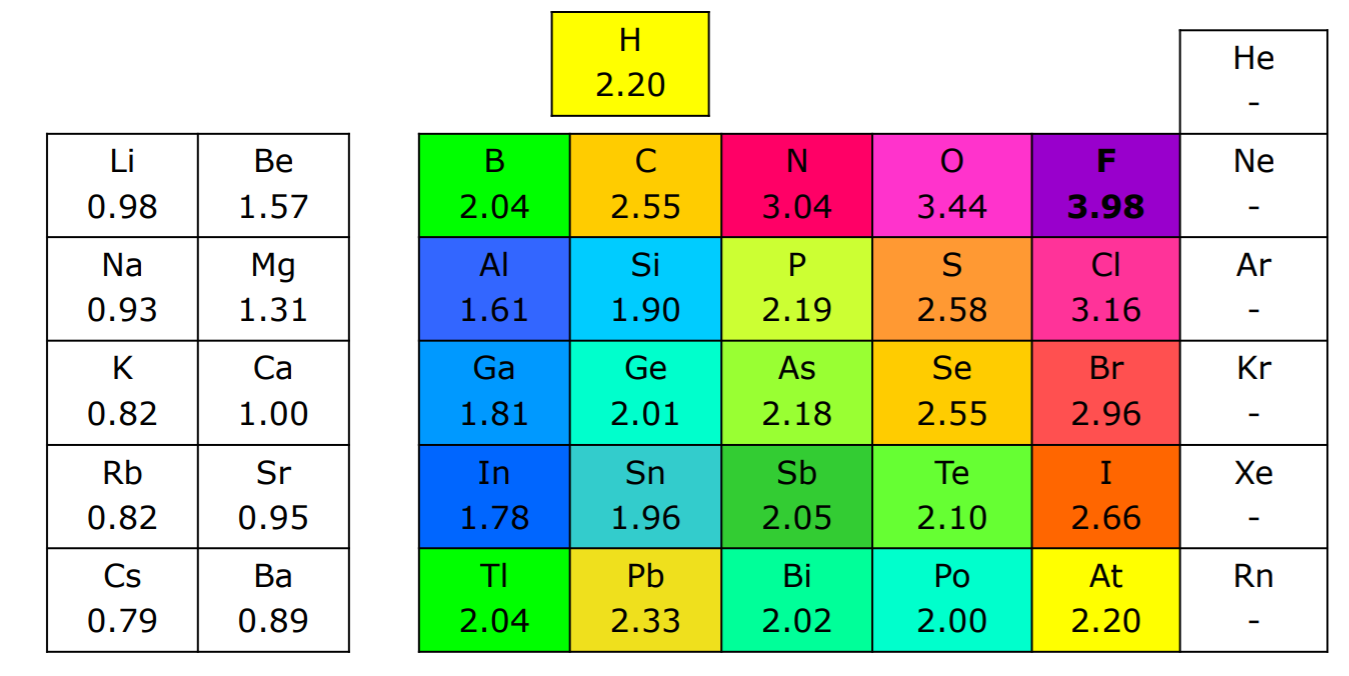
\includegraphics[width=10cm]{pauling.png}
    \end{figure}

    The electronegativity across the p-block is relatively trendy, increasing across a period and down a group,
    once again all the metalloids have a similar electronegativity. The jump in periods 4 and 5 from 3 in groups
    13 and 14 is from the d and f orbitals which provide weak shielding, giving them a higher effective nuclear 
    charge. Electronegativity varies depending on the hybridisation, sp \(>\) sp \(^2\) \(>\) sp\(^3\).
    \begin{figure}[h]
        \centering
        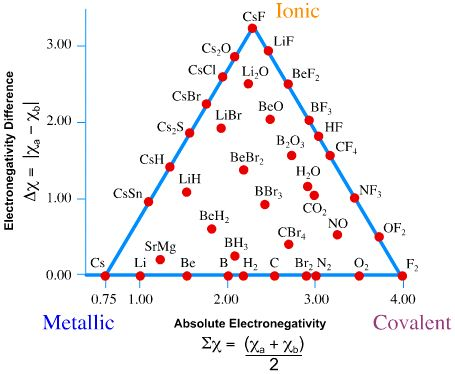
\includegraphics[width=8cm]{triangle.jpg}
    \end{figure}
    The van Arkel Ketelaar triangle is valid for simple sp compounds. 

    \subsubsection{Summary}
    \begin{itemize}
        \item Ionisation energies increase left to right and decrease top to bottom
        \item Electron affinities broadly increase left to right
        \item Electronegativity increases left to right and decreases top to bottom
    \end{itemize}
    Further reading: Inorganic Chemistry (M. Weller, T. Overton et al) (7th edition) sections 1.7 and 2.13
    \newpage

    \subsection{Effective Nuclear Charge}\thedate{28/10/20 --- Week 1}
    \subsubsection{Slater's Rules}
    There is a trendy decrease moving across each period and a trendy increase moving down each group.
    \begin{figure}[h]
        \centering
        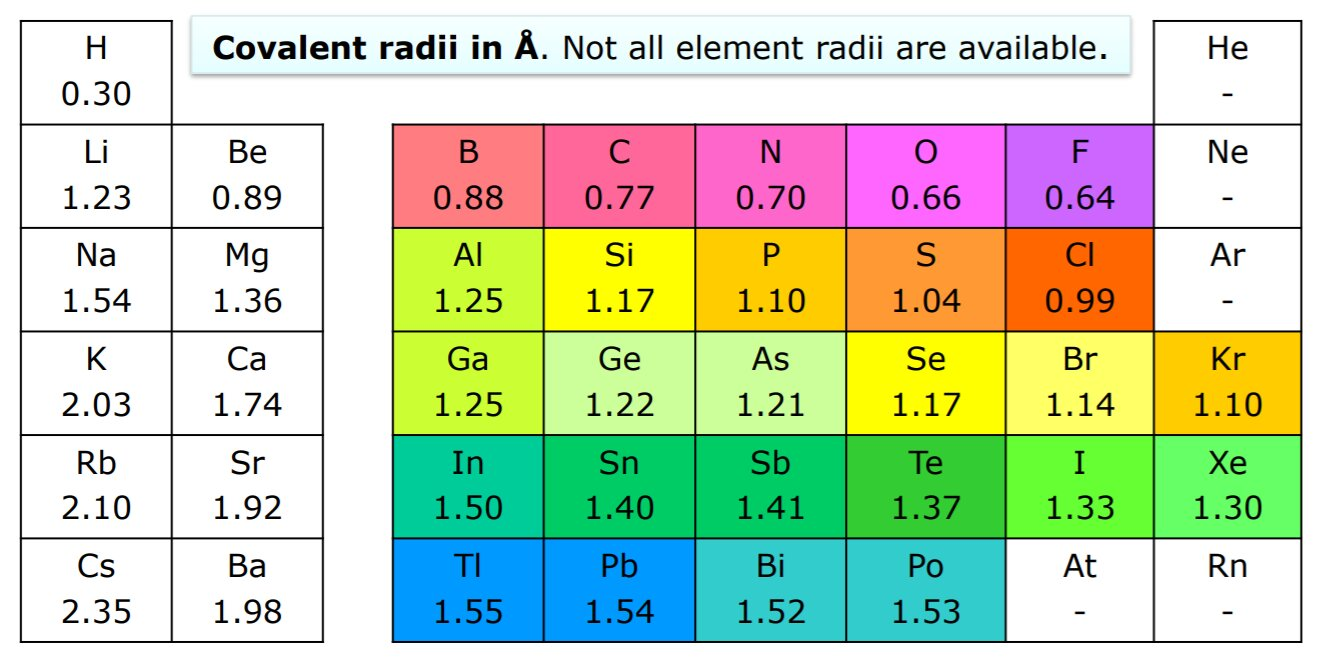
\includegraphics[width=10cm]{covrad.jpg}
        \caption{Covalent radius}
    \end{figure}

    Slater's rule: the outermost electrons `feel' a nuclear charge which is less than the actual charge because
    of shielding effects (s) from other electrons. \(Z^* = Z - s\) (\(Z^*\) is sometimes called \(Z_{\text{eff}}\))

    We can calculate the shielding constant (s) through simple calculations. 
    \begin{enumerate}
        \item Write out the electronic configuration in the following way:
        
        (1s), (2s, 2p), (3s, 3p), (3d), (4s, 4p), (4d), (4f), (5s, 5p) etc.

        \item When considering a particular electron in an ns or np orbital:
        
        Each electron with the same principal quantum number i.e. (ns, np), (nd) contributes 0.35\\
        Each electron in the (n-1) shell contributes 0.85\\
        Each electron in the (n-2) or lower shells contribute 1.00 

        \item When considering a particular electron in an nd or nf orbital:
        
        Each of the other electrons in the (nd, nf) group contributes 0.35\\
        Each of the electrons in a lower group than the one being considered contributes 1.00\\
    \end{enumerate}
    \NB Do \textbf{NOT} include the electron that you are considering when calculating \(s\), it cannot shield the
    nucleus from itself.

    \begin{figure}[h]
        \centering
        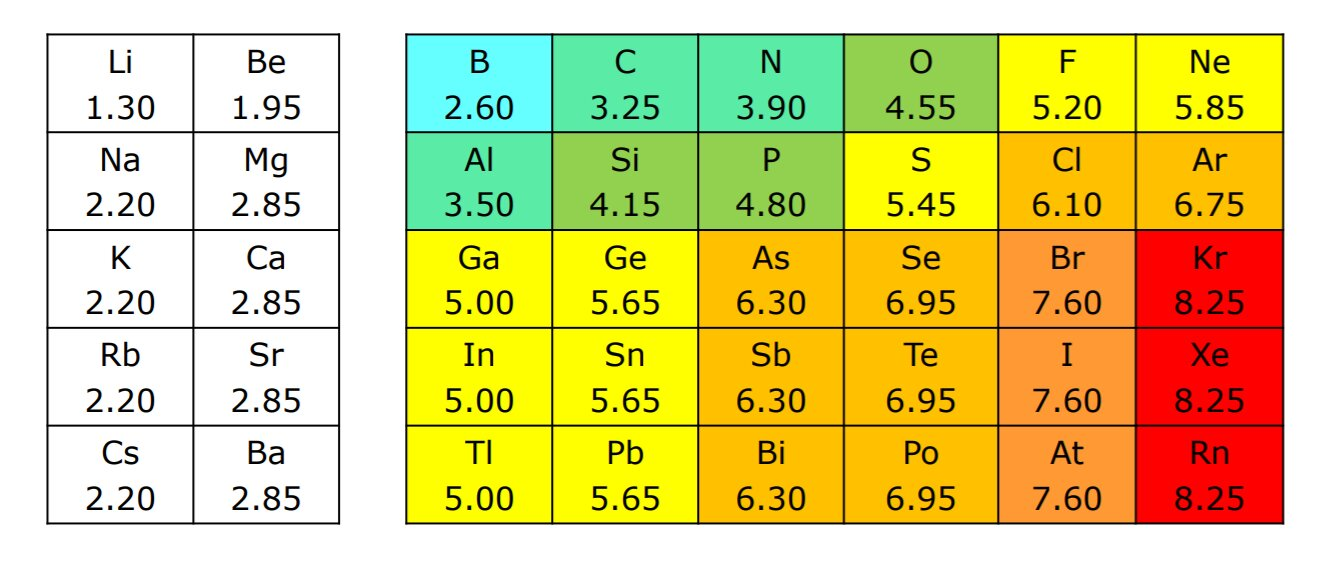
\includegraphics[width=10cm]{eff.jpg}
        \caption{Effective nuclear charge}
    \end{figure}

    The effective nuclear charge increases across a period and down a group. The values begin to flatten out at
    the bottom periods, this is because (n-2) contribtues 1.00 to s. 
    \newpage
    \begin{figure}[h]
        \centering
        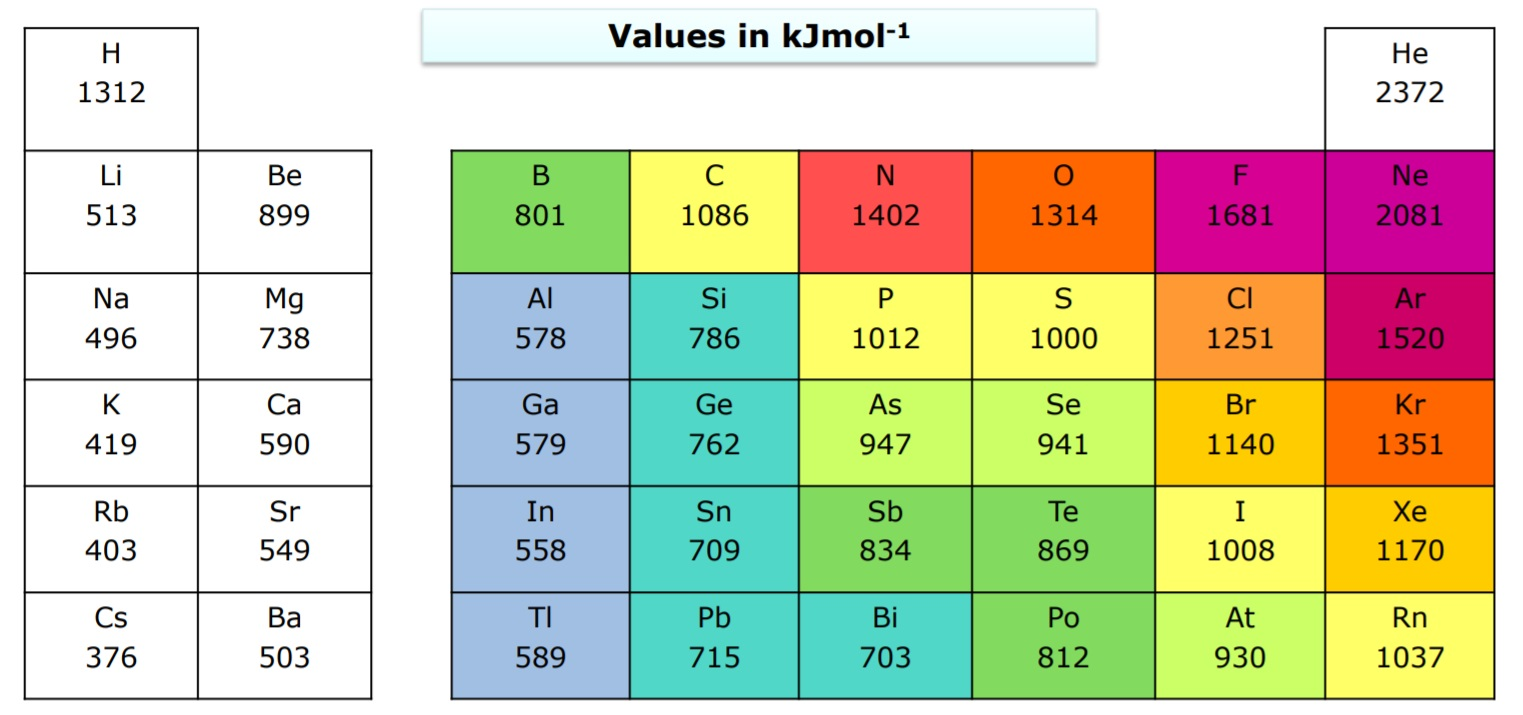
\includegraphics[width=10cm]{ionisation energy.jpg}
        \caption{Ionisation energy}
    \end{figure}

    Despite this flattening off the ionisation energy decreases down the groups (except for 13), this is because
    the radius is also an important factor for determining ionisation energy.

    \begin{figure}[h]
        \centering
        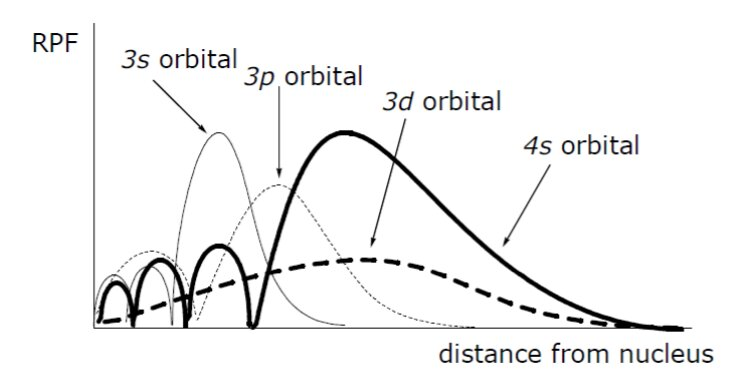
\includegraphics[width=10cm]{pen.jpg}
        \caption{RPF is the probability of finding it there}
    \end{figure}

    Slater's rules are very simplistic and can only explain the increase across period in ionisation energy, it 
    cannot explain the reduction in ionisation energy down a group. This is because it does not take into account
    the penetration of higher principal quantum number electrons. When a 4s electron is closer to the nucleus 
    it will feel more charge.
    \newpage
    \subsubsection{Covalent and Ionic Radii}

    A covalent radius is defined as half the length of a symmetrical homonuclear element bond (X-X)

    \begin{figure}[h]
        \centering
        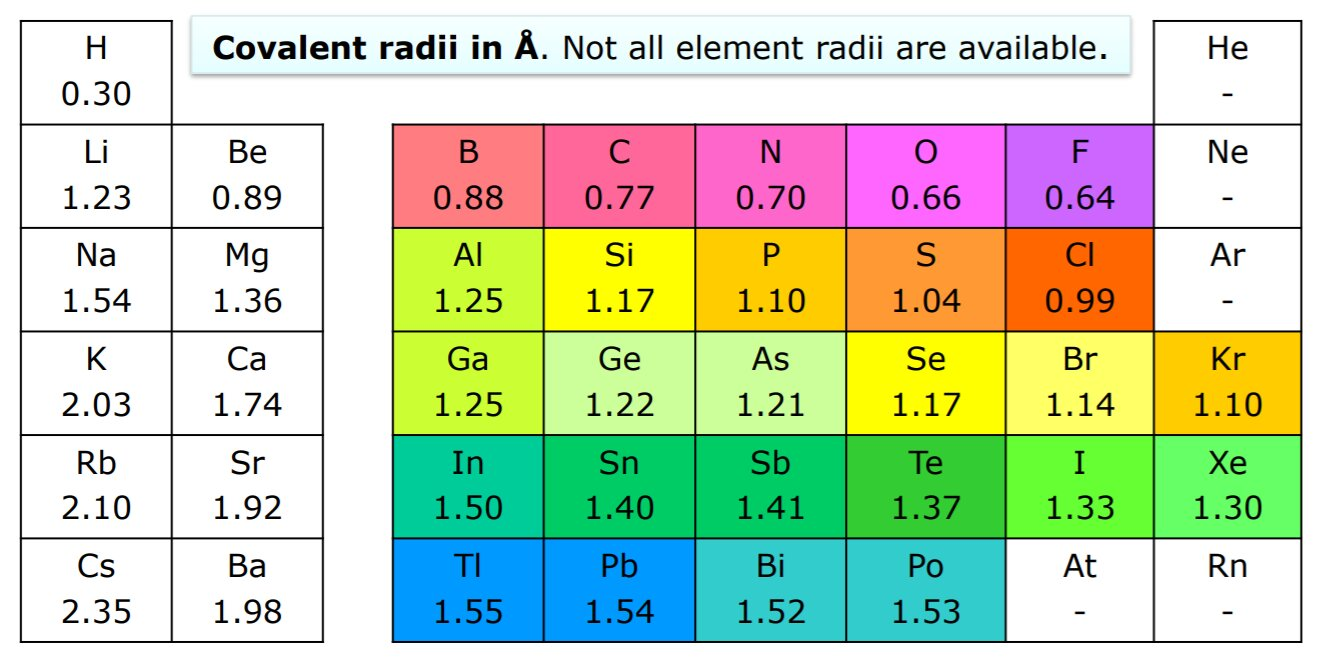
\includegraphics[width=10cm]{covrad.jpg}
        \caption{Covalent radius}
    \end{figure}

    \NB Bonds will shorten if ionic character is present, so we must account for electronegativity differences.

    Make this itemized.
    There is a decrease across a period as effective nuclear charge increases, the nuclear charge increases by 1
    whilst only decreaseing 0.35 from ony more p-electron. Radii increases down a group as the valence electrons
    are in the next principal quantum shell so they're further from the nucleus (Slater's rules cannot account
    for this). Obviously anions are large because of more inter-electron repulsion and cations are smaller because
    of a less repulsion. Thusly a higher oxidation state means a higher effective nuclear charge.
    Radii will also vary depending on the coordination number (ligands giving electron density).

    \subsubsection{s-p energies}

    \begin{figure}[h]
        \centering
        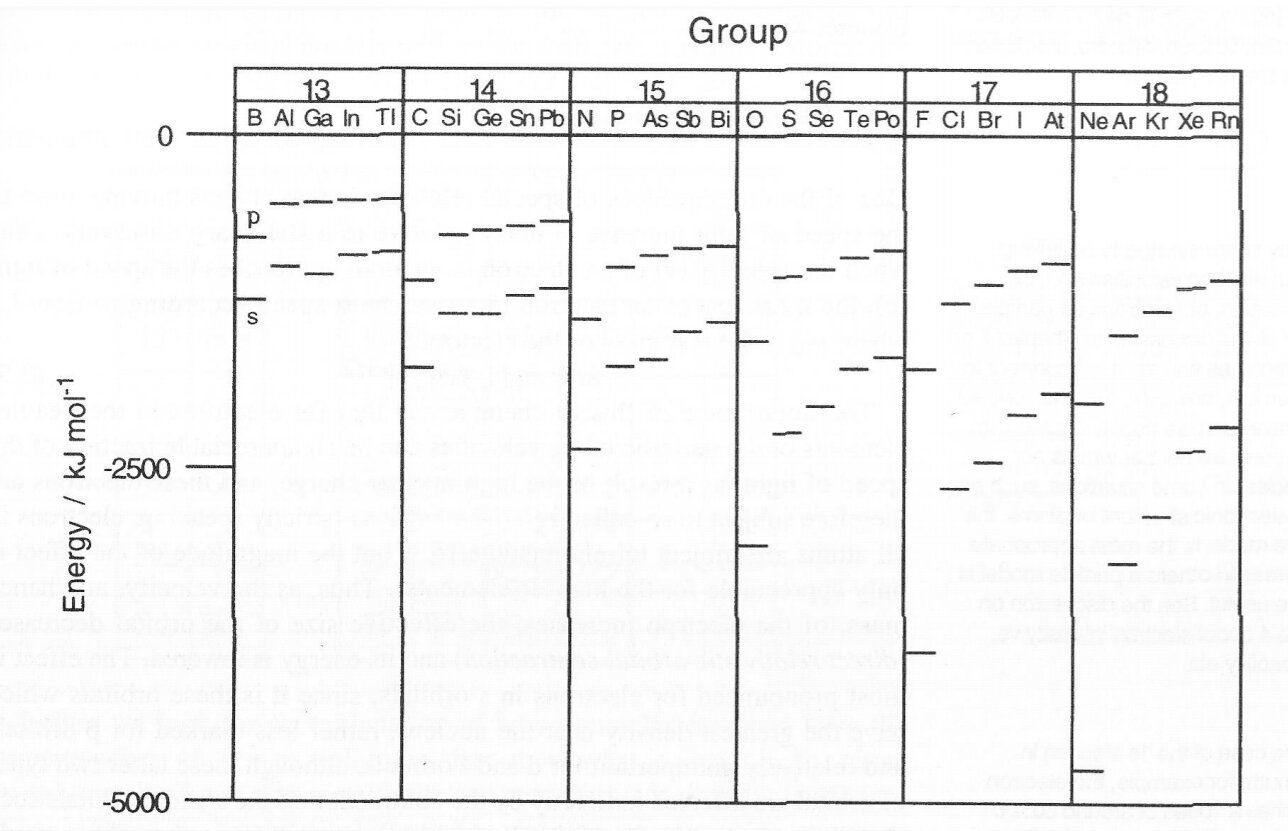
\includegraphics[width=10cm]{s-psep.jpg}
        \caption{Highest occupied orbital energies}
    \end{figure}

    Down a group the s \& p orbitals increase (less negative) in energy and the s-p energy separation decreases.
    The higher principal quantum shell electrons are further away from the nucleus and so the pull is less
    and the s cannot penetrate as far inside, making s \& p closer together and giving a less negative energy 
    for both (it's easier for the electron to leave). Ga and Ge deviate from this trend, once again
    this is from the 3d orbital preceding them, thus decreasing the energy of the s orbitals as they can penetrate
    further into the 3d orbital, making the s orbital more evenly distributed. (I don't if this is right, he said something about an s orbital being more evenly 
    distributed? \textbf{Check this out later.}) The 4s orbital for As, Se, Br and
    Kr are lower than expected. This is because of the increased \(Z^*\) from their higher proton count having a strong
    effect on the 4s electrons which allow it to penetrate further into the core.  

    The distance between s \& p increases and the energy decreases as 
    we go across a period. Due to a better \(Z^*\) and more penetration for s. This is why the \(\sigma\) and \(\pi\)
    levels swap around from N\(_2\) to O\(_2\) due to s-p mixing: 
    For Li \(\ce{->}\) N (three or fewer electrons in the p orbitals) the s-p orbitals are close together and so
    can mix, mathematically the \(\sigma_{s}\) and \(\sigma_{p}\) wavefunctions combine (influence each other) with the result that the 
    \(\sigma_{s}\) orbital becomes more stable and the \(\sigma_{p}\) becomes less stable, similarly their antibonding orbitals also
    follow the same trend. This causes the \(\sigma_{p}\) to switch places with the degenerate(same energy levels) \(\pi_{p}\)
    molecular orbitals. (Molecular Orbitals from 1st year). 

    \begin{figure}[h]
        \centering
        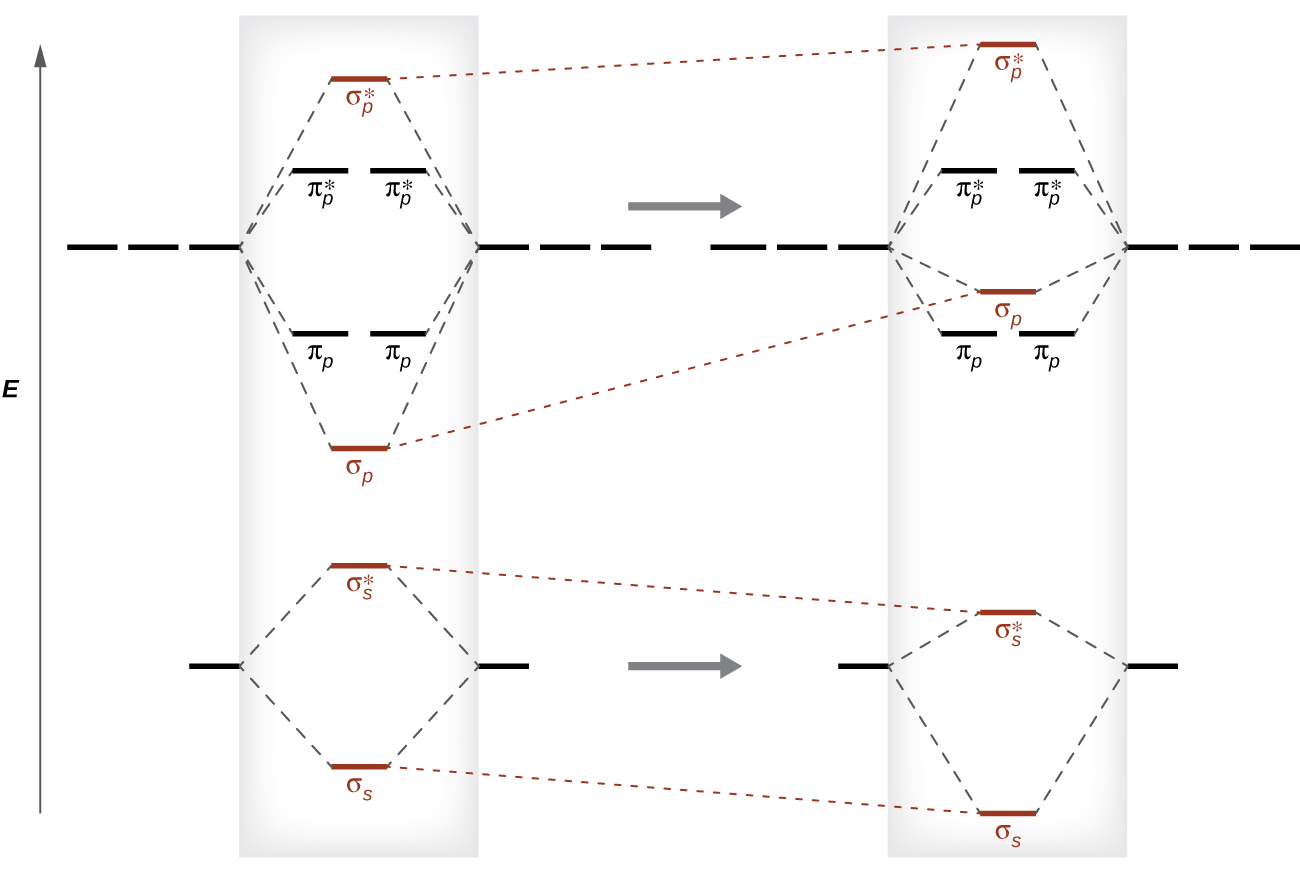
\includegraphics[width=10cm]{MO.jpg}
        \caption{MO shape of Oxygen(left) and Nitrogen(right)}
    \end{figure}

    \begin{figure}[h]
        \centering
        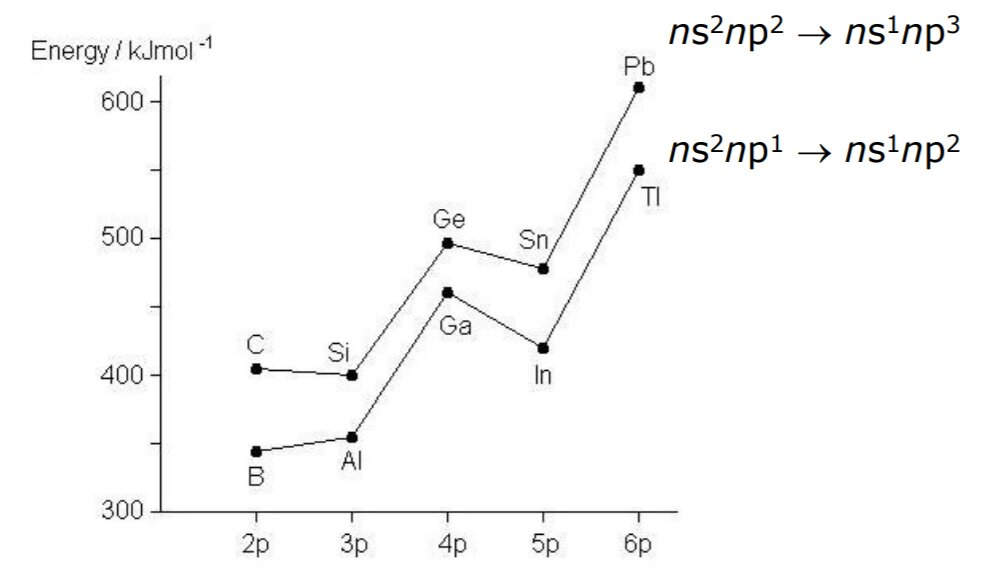
\includegraphics[width=10cm]{trans.jpg}
        \caption{Reorganisation energies of groups 13 and 14}
    \end{figure}

    As we go down a group the energy to promote an s electron to a p-orbital increases, with the sharp execption of 
    Ge and Ga, as the 4s orbital is preceded by a 3d row, so the energy of the 4s orbital is lower (more stable). 
    Unexpectedly Ti and Pb have the highest promotion energy, this has substantial implications on hybridisation
    energies. Remember when an electron moves the others do not stay static, their energies change due to
    electron correlation.
    \newpage
    \subsection{Inert Pair Effect}

    We can see that when we change the electronegativity of the bonded atom (from Oxygen to Fluorine) it changes
    the boundry of when we have a discrete covalent molecule and when we have a network structure, like in the
    van Ketelaar triangle. We can see that with the more electronegative Fluoride it favours covalent bonds more.

    \begin{figure}[h]
        \centering
        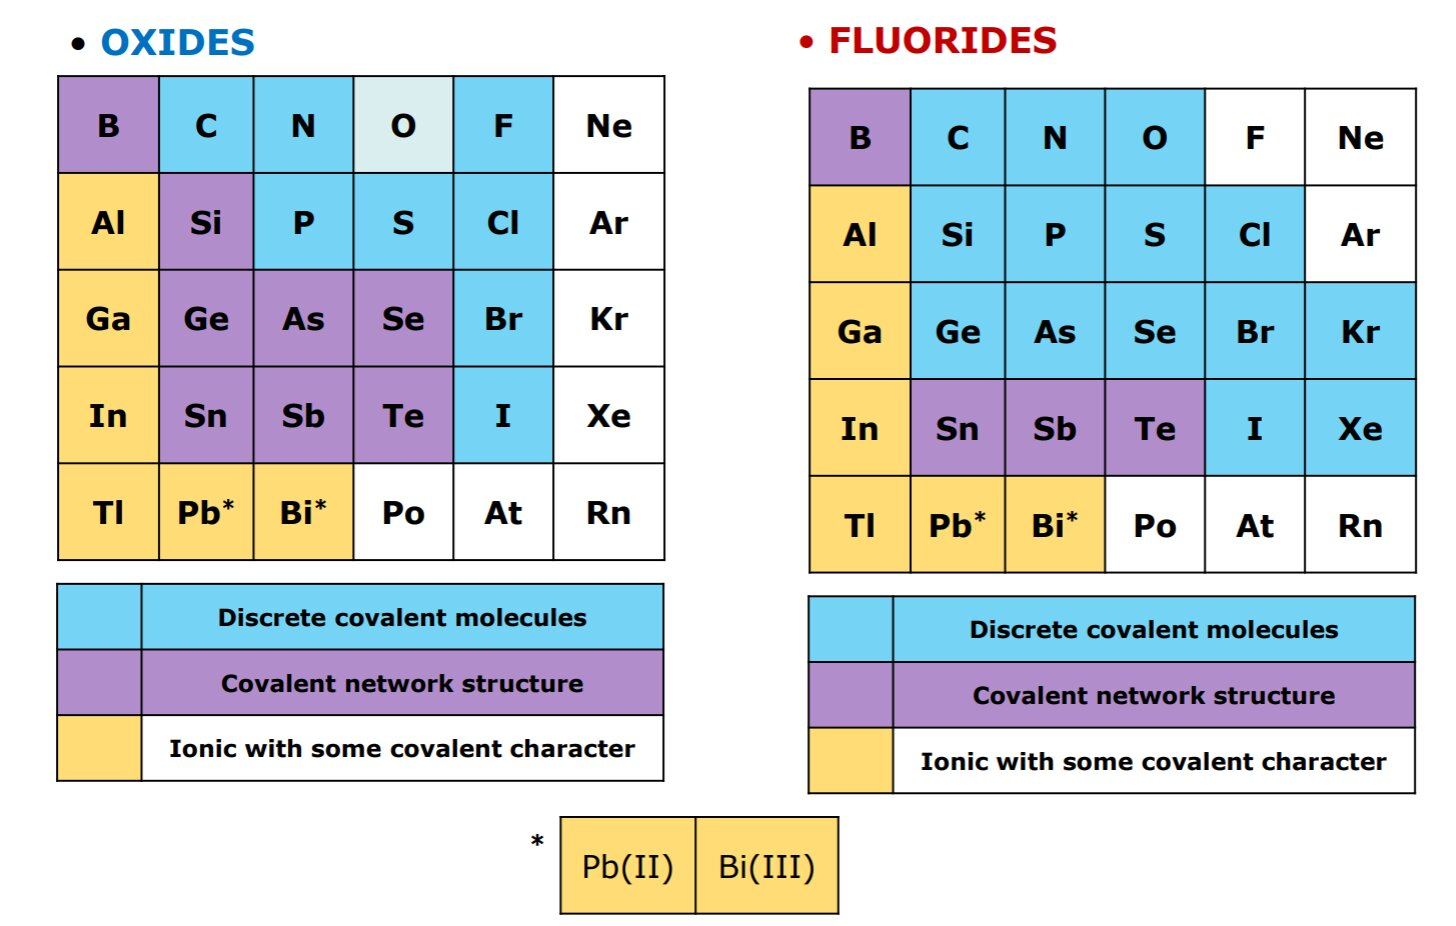
\includegraphics[width=10cm]{of.jpg}
    \end{figure}
    \NB Covalent network structures are like diamonds.\\

    These trends are governed by electronegativity differences, Indium has a much lower negativity than Xenon,
    and so has less oxidation states. This is generally more trendy higher up on the periodic table, whereas 
    elements in the lower periods may perfer lower oxidation states. 

    \begin{figure}[h]
        \centering
        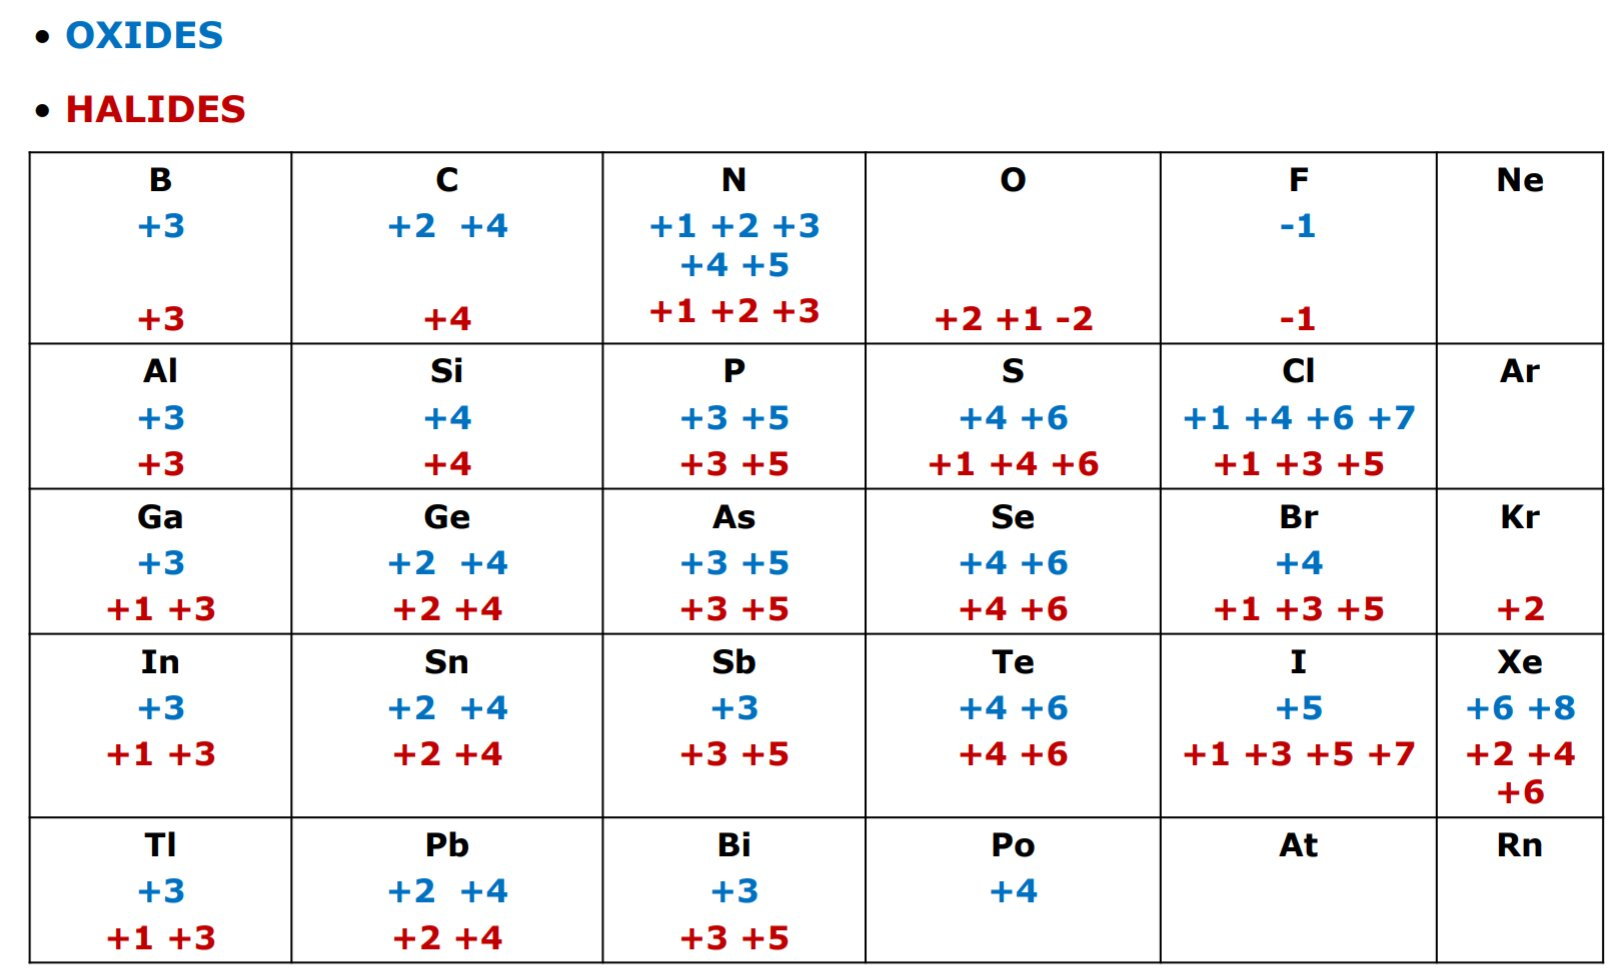
\includegraphics[width=10cm]{ox.jpg}
    \end{figure}

    The inert pair effet is the tendency of electrons in the outermost s orbital to remain unionised or unshared
    in the compounds of group 13-16 elements. 

    The most common oxidation state for group 13 is +3, however +1 is common for Tl (at the bottom of group 13).
    The stabibility for group 13 is Al $<$ Ga $<$ In $<$ Ti going down the group. Why is this? No one knows.
    We can guess and say that the relativistic effects are stabilising the 6s orbital of Tl. More importantly the strength
    of the covalent bonds also decrease down a group due to poor orbital overlap. This resulsts in the bond
    enthalpy not offsetting the rehybridisation energy cost. (i.e. it costs more energy to form an sp3 orbital
    for Pb than would be in the Pb-C bond and so is not energetically favourable.)\\

    Look at the figure below, as you can see with two small atoms the overlap of their s orbitals is very effective,
    both have large amounts of electron density overlapped. However with the small-big case, the big one has a very
    tiny amount of electron density in the small region, so the overlap is poor.

    \begin{figure}[h]
        \centering
        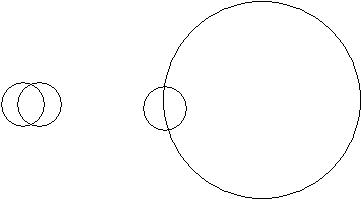
\includegraphics[width=4cm]{over.jpg}
        \caption{overlap of atoms helps to determine bond strength}
    \end{figure}

    In Bi the 1s electron reaches 60\% c, thus m = 1.26 (relativistic effects), so the 1s orbital contracts
    by 20\% thus lowering its energy. This is called direct relativistic orbital contraction.

    The s orbitals penetrate most and so are more stabilised (less available for bonding). p orbitals contract
    much less due to poorer penertration and so are more available for bonding. 

    d and f orbitals experience indirect relativist orbital expansion (destabilised). Their poor penertration and
    the contraction of the s and p electrons leaves them more shielded and less affectedby Z*.

    \subsection{Multiple bonding}
    Generally as we go down the groups the bonds become weaker, the orbitals are more diffuse and the bonds
    are longer. 

    In the first row the 2p\(_\pi\) orbitals are use in multiple bonding, they have a good overlap due to a short
    bond length, despite having a smaller covalent overlap.
    In the second row and beyond the larger covalent radius is cancelled out by the much larger bond length, so
    there is no common multiple bonding.

    \begin{figure}[h]
        \centering
        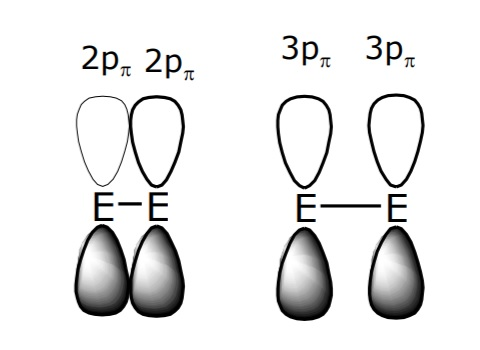
\includegraphics[width=6cm]{ov.jpg}
    \end{figure}

    \begin{center}
        \begin{tabular*}{4cm}{l l l}
            C=O & C-O & \(\Delta\pi\)\\
            715 & 335 & 380 kJ mol\(^{-1}\)\\
            S=O & Si-O & \(\Delta\pi\)\\
            590 & 420 & 170 kJ mol\(^{-1}\)
        \end{tabular*}
    \end{center}

    So we can see that Si which is down a period from C has half of the stabilisation energy from a double bond.
    Thus the single bonded Silicone Oxide is more stable, unlike Carbon, where the p\(_\pi\)-p\(_\pi\) overlap
    stabilises the bond.

    % \chemfig{C(-[0]O)(-[2]O)(-[4]O)(-[6]O)} 2x715 = 1430 \chemfig{C(=[0]O)(=[4]O)} 4x335=1340 \(\sigma + \pi\) is stable
    \begin{figure}[h]
        \centering
        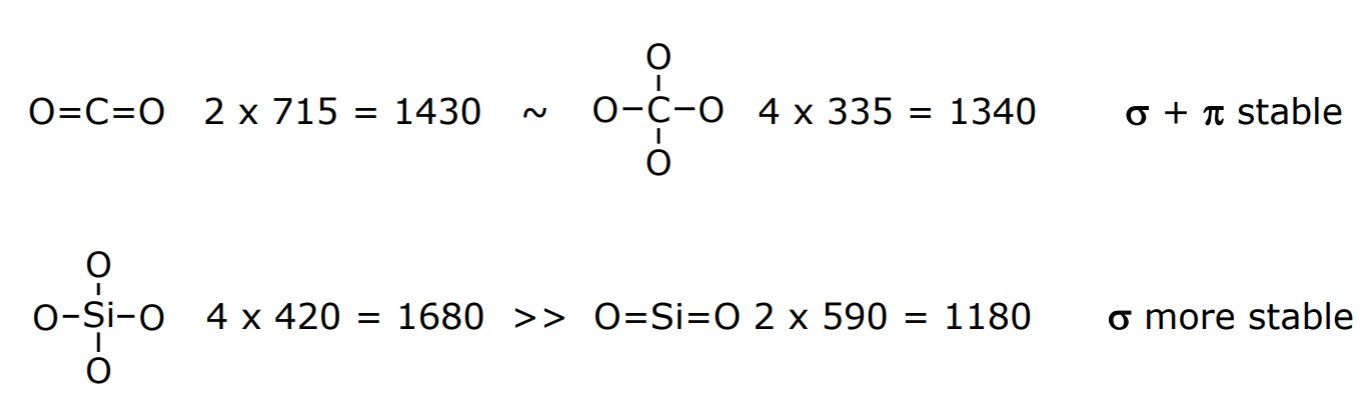
\includegraphics[width=10cm]{stab.jpg}
    \end{figure}
    \newpage
    \subsubsection{p\(_\pi\)-d\(_\pi\) overlap}
    A filled p-orbital can donate to a vacant d-orbital that is pointing in its directions. More dispersed 
    so can reach over the longer bond, this is called d-p \(\pi\) back bonding or p\(_\pi\)-d\(_\pi\) bonding (very confusing, I know).
    One example of this is the P=O beond, the O back bonds to the vacant d-orbital on the P atom, giving a 
    double bond from the \(\pi\) bond formed.
    % two images side by side
    \begin{figure}[h]
        \centering
        \subfloat[\centering]{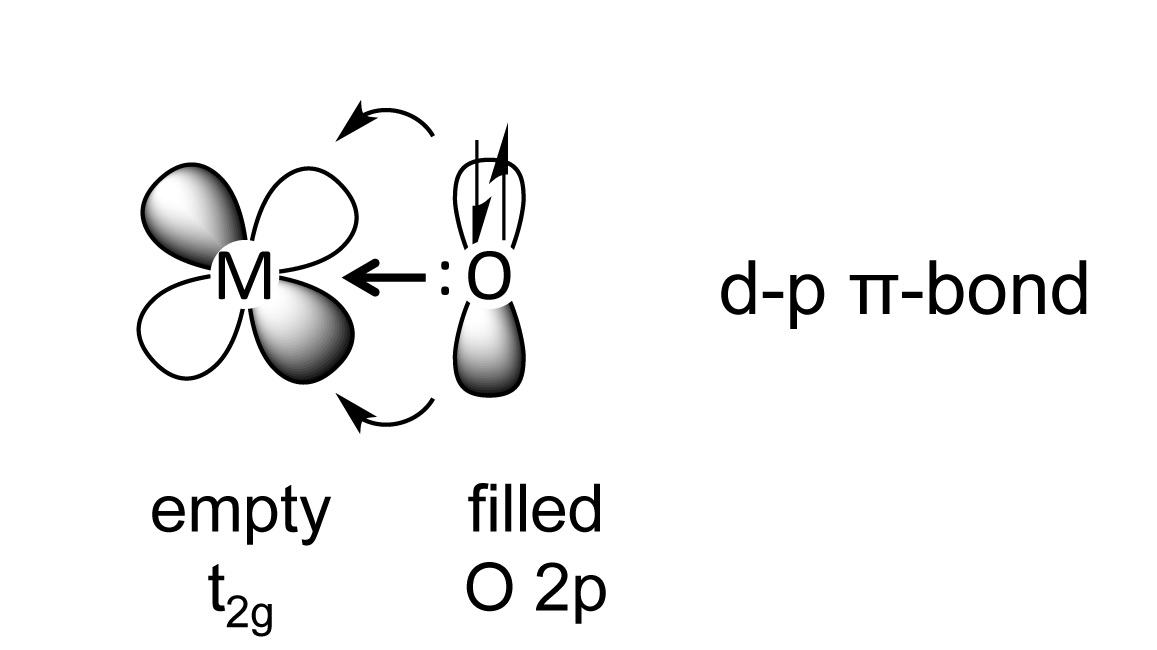
\includegraphics[width=8cm]{d-p.jpg}}
        \qquad
        \subfloat[\centering]{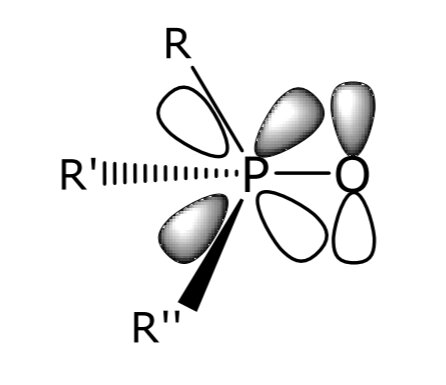
\includegraphics[width=6cm]{po.jpg}}
    \end{figure}

    \begin{tabular*}{100cm}{l l l l l l}
        & CCl\(_4\) & SiCl\(_4\) & GeCl\(_4\) & SnCl\(_4\) & PbCl\(_4\) \\
        \(\Delta H\deg_f\) kJmol\(^{-1}\) & -107 & -628 & -510 & -493 & -284\\
        M-Cl kJmol\(^{-1}\) & 326 & 402 & 339 & 314 & ---\\
    \end{tabular*}
    \vspace{2cm}
    \(\Delta H\deg_f\) of Si is greater than C because of the ionic contribution to the Si-Cl bond (Si is 
    less electronegative). Then as the orbitals become bigger and overlap becomes 
    poorer \(\Delta H\deg_f\) falls, as does the M-Cl bond energy.  

    CCl\(_2\) and SiCl\(_2\) do not exist, because it is more energetically favourable to hybridise and form 
    their trichlorides instead. But GeCl\(_2\) does exist, due to the 3d shielding effect on the 4s which allows
    it to bond like that, GeCl\(_4\) also exists. PbCl\(_2\) is more stable than PbCl\(_4\) because of relativistic
    effects and the inert pair effect.

    \subsection{The Triels}\thedate{Week 3}
    
    \vspace{0.4cm}
    Consisting of Group 13. They have the general config of ns\sup{2}np\sup{1}. So their chemistry is dominated
    by electron deficiency, they have fewer valence electrons than the number of vaence orbitals (two completely empty p orbitals). 
    They form Lewis acids.
    
    EX\sub{3} e.g. BF\sub{3} has 6 valence electrons, so it accepts an electron from a Lewis base. 
    AlCl\sub{3} is useful for Fieldel Crafts reactions, it actually forms a dimer as the lone pair of electrons
    on the Cl forms a dative bond with the other aluminium atom. However in reality the bonds are delocalised around
    the ring. 
    \begin{figure}[h]
        \centering
        \subfloat[\centering]{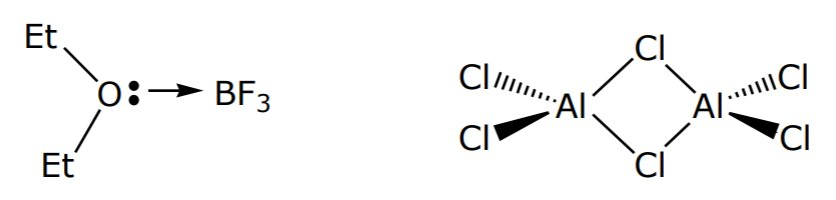
\includegraphics[width=6cm]{dat.jpg}}
    \end{figure}
    \begin{itemize}
        \item EX has 4 valence electrons is most stable for Tl (but not when X = H). 
        \item Boron clusters also form EX, (X = H, Cl)
        \item For AlX and GaX they diproportionate: \ce{3MX -> 2M + MX\sub{3}}
        \item The +1 oxidation state becoems more stable as the group descends.
    \end{itemize}
    This descending trend is because of the inert pair effect, the tendency of electrons in the outmermost s orbital to 
    remain unionised or unshared in compounds of group 13-16.

    \subsubsection{Boron Chemistry}
    BX\sub{3} exists for all Halogens. BF\sub{3} can participate in $\pi$ bonding.
    The B-F bond is very short so there is some overlap between the vacant p-orbital in Boron and the spare electron
    pair in Fluoride, so there is some $\pi$ bonding characterists in BF\sub{3}. Although the bond is not strong
    because of the large electronegativity difference, it still has influence on the properties of BF\sub{3}

    \begin{figure}[h]
        \centering
        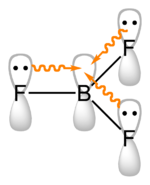
\includegraphics[width=2cm]{bf3.png}
    \end{figure}

    Lewis acid strength: BI\sub{3} $>$ BBr\sub{3} $>$ BCl\sub{3} $>$ BF\sub{3}.
    This is due to longer bonds, and so the overlap between the p-orbitals is lesser. Thus the vacant Boron 
    p-orbital can better accept a lone pair of electrons. 

    We know that the non-Fluoride halides for the other triels dimerise e.g. AlCl\sub{3} to Al\sub{2}Cl\sub{6}.
    This is due to a poor overlap of Cl and Al due to the large orbitals, so dimerisation is preferable to $\pi$ bonding.

    BX\sub{3} undergo exchange reactions. 
    \begin{figure}[h]
        \centering
        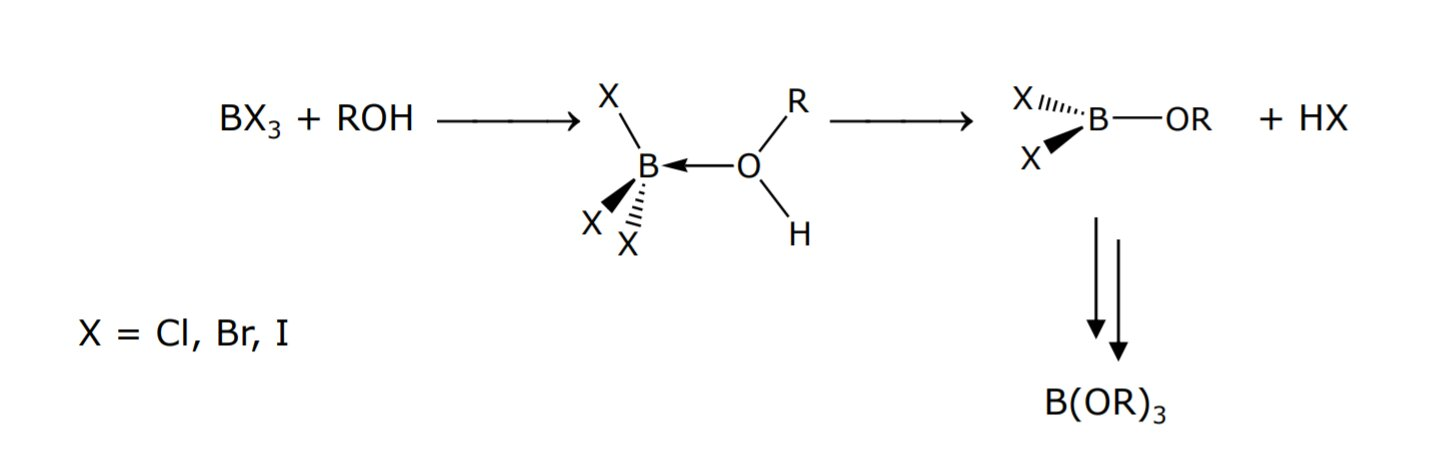
\includegraphics[width=10cm]{ex.jpg}
    \end{figure}

    This does not happen to BF\sub{3} because the B-F bonds are too strong, instead it acts as a catalyst.
    Low acidity but high stability. 

    If we compare the stability of the acid-base(\textbf{L}) complex for  of Al, Ga, In we see:
    
    MF\sub{3}\textbf{L} $>$ MCl\sub{3}\textbf{L} $>$ MBr\sub{3}\textbf{L} $>$ MI\sub{3}\textbf{L}. This is the opposite
    for B. This is becaue of the longer bonds and so no $\pi$ back bonding. MF\sub{3} is a stronger lewis acid as 
    fluride is very electrowidthdrawing and so that makes the vacant p-orbital on the triel more electronegative
    making it easier to accept a pair of electrions.

    \begin{figure}[h]
        \centering
        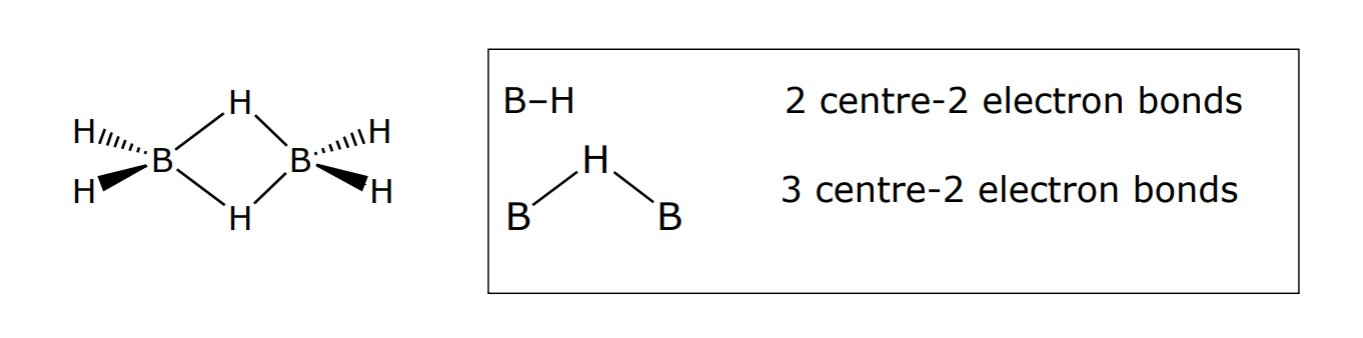
\includegraphics[width=10cm]{b2h6.jpg}
    \end{figure}

    Boron Hydries (Boranes), BH\sub{3} cannot $\pi$ bond with H as it has no lone pairs, so it forms an electron
    deficient dimer. Valence bond theory cannot account for this structure as there are not enough valence electrons.

    The B sp\sup{3} hybridises but with an empty electron instead. There is then overlap between the empty sp\sup{3} B 
    orbital, a filled sp\sup{3} orbital and the 1s electron, this forms a banana bond

    \begin{figure}[h]
        \centering
        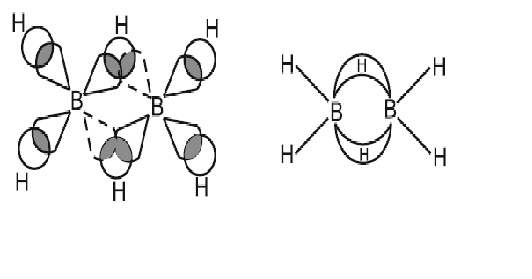
\includegraphics[width=6cm]{ban.png}
    \end{figure}

    \begin{figure}[h]
        \centering
        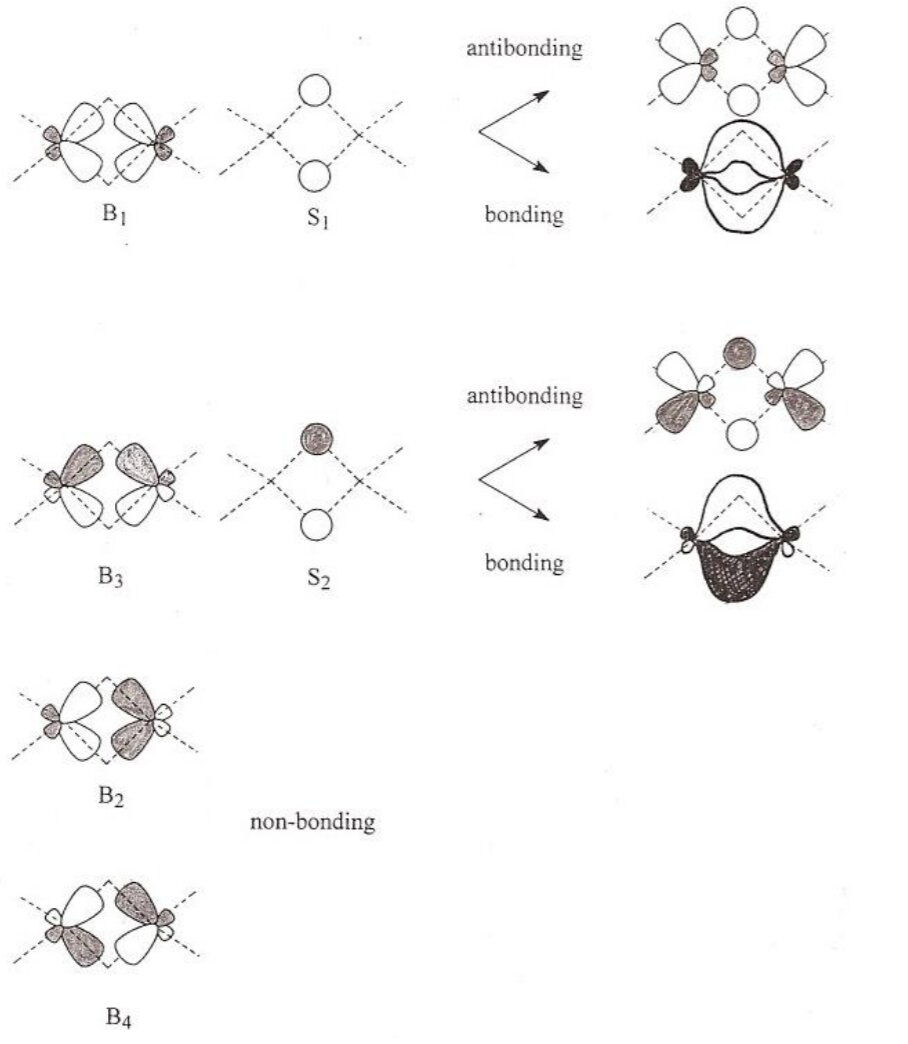
\includegraphics[width=6cm]{bmo.jpg}
    \end{figure}

    The different colours represent the different \emph{phases} of the electrons. They all need to be of the same phase
    to form a bond together. They need to have the same \emph{symmetry}. You need to go over MO again, idiot.

    Hydries become less stables as the group descends, Gallane was only discovered in 1989.
    In\sub{3} and Tl\sub{3} are too unstable to exist unless they are coordinated with a Lewis base. 

    Aluminum compounds are more stable when substituted with alkyls e.g. AlR\sub{2}H, they form stable dimers.

    Aluminum hyrides and borohydrides are very good at reducing. 

    \newpage

    \subsection{Wade's Rules}\thedate{Week 3}

    Rules to predict the structure of Boron hydrides (B\sub{n}H\sub{m} or anions of that B\sub{n}H\sub{m} \sup{x}\sup{-})
    by counting the number of electron pairs for cluster bonding.

    \begin{enumerate}
        \item Each B-H unit donates two electrons (one pair) to cluster bonding.
        \item Any additional hydrogen atoms i.e. not bonded to Boron, donates one electron to cluster bonding.
        \item Add the overall charge of the molecule e.g. 2 extra electrons for a 2\sup{-} charge
        \item Add up the total number of electrons, should be even, so there are 2n in total, meaning n pairs of electrons involved in cluster bonding.
        \item If we have n pairs then the structure is based around a polyhedron with n-1 vertices. e.g. 7 pairs means a 6 vertexed polyhedron which is an octahedron.
        \item Count the number of B-H units.
        \begin{itemize}
            \item If B-H = number of vertices (n-1) then place one B-H unit at each vertex, this structure is described as \textbf{CLOSO}, CLOSED, there is no open face.
            \item If B-H is one fewer than the number of vertices, B-H - 1 = n-1, then places B-H units at all but one of the vertices, this structure is described as \textbf{NIDO}, NEST.
            \item If the number of B-H units is two fewer than the number of vertices, B-H - 2 = n-1, then fill all but two of the vertices (these two vertices must be adjacent), the structue is described as \textbf{ARACHNO}, COBWEB.
        \end{itemize}
        \item Place any remaning hydrogens as bridging Hs around the open face. If there are any left then place them on the electron deficient boron atoms around the open face, they are the ones that have 'lost' the most bonds from the original \textbf{CLOSO} structure.
    \end{enumerate}
    
    Wade's Rules can also apply for different atoms by treating them as BH groups

    \begin{tabular}{l l}
        C, Si, Ge, Sn & BH\\ 
        N, P, As & \ce{BH_2}\\
        S, Se & \ce{BH_3}
    \end{tabular}

    \begin{figure}[h]
        \centering
        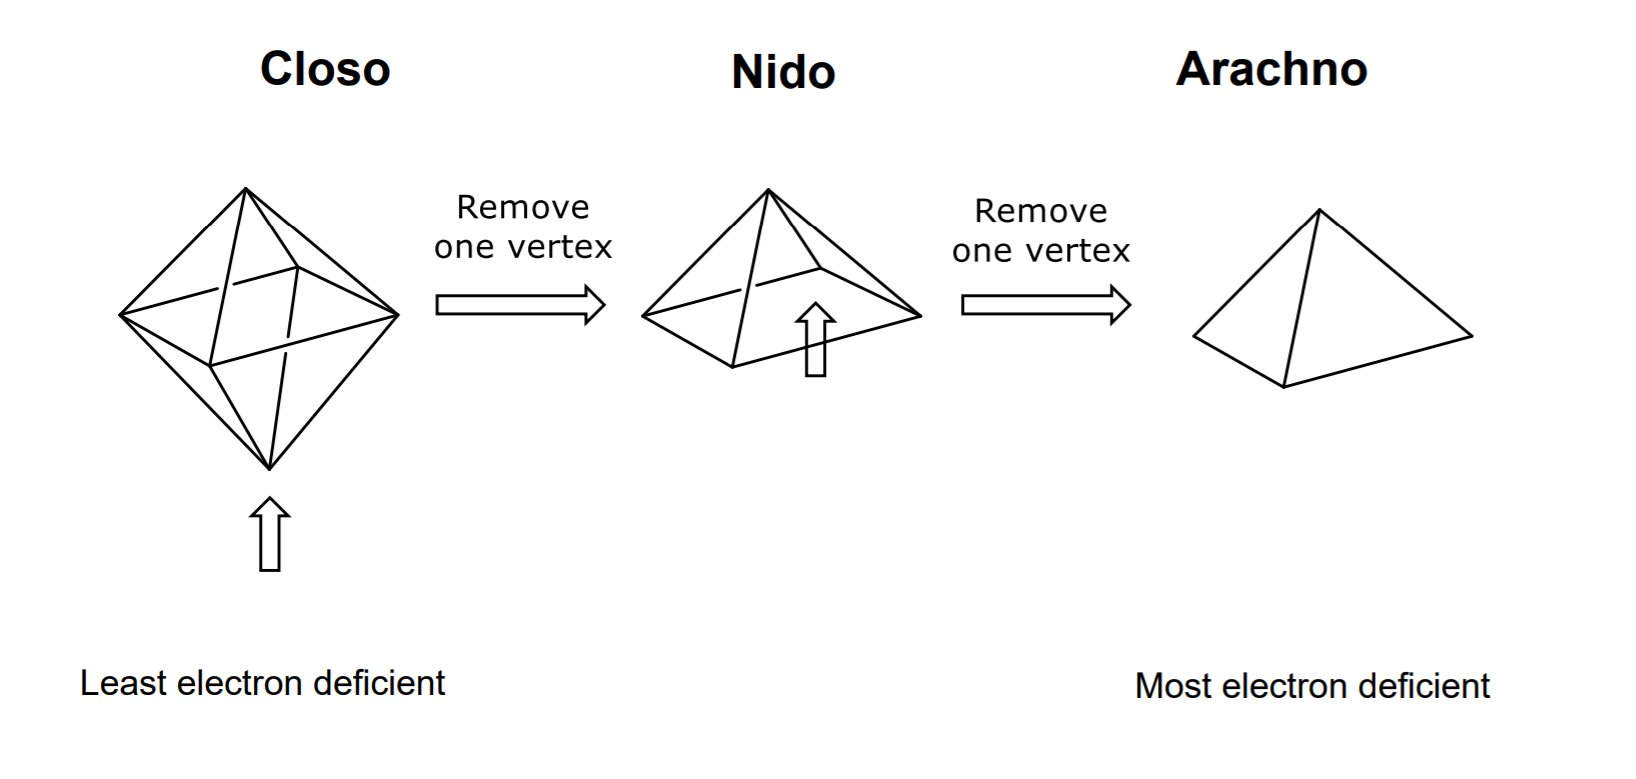
\includegraphics[width=10cm]{closo.jpg}
    \end{figure}

    Learn from an example. B\sub{6}H\sub{6}\sup{2}\sup{-}
    
    \begin{itemize}
        \item B\sub{6}H\sub{6}\sup{2}\sup{-} = (BH)\sub{6}\sup{2}\sup{-} = six B-H units, six pairs of electrons
        \item Number of electrons available for cluster bonding = 14 = 6*2 (from B-H units) + 2 (from the 2 minus charge)
        \item 14 electrons in total so n = 7 pairs.
        \item n-1 = 6, meaning 6 vertices which gives us an octahedron.
        \item Count the number of B-H units, six, this is the same as n-1, which means we have a \textbf{CLOSO} structure, and one B-H fragment at each vertex.
        \item We have no extra hydrogens so the structure is complete.
    \end{itemize}

    \begin{figure}[h]
        \centering
        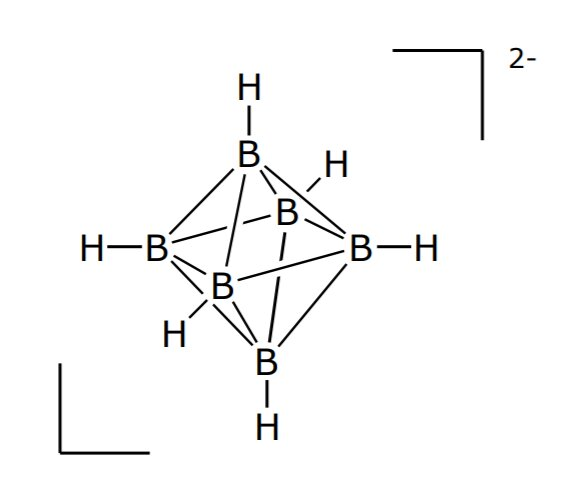
\includegraphics[width=6cm]{boro.jpg}
    \end{figure}

    \newpage

    A second example. B\sub{4}H\sub{1}\sub{0}
    
    \begin{itemize}
        \item B\sub{4}H\sub{1}\sub{0} = (BH)\sub{4}H\sub{6} = four B-H units and six hydrogens.
        \item Number of electrons available for cluster bonding = 14 = 4*2 + 6.
        \item 14 electrons in total so n = 7
        \item n-1 = 6, 6 vertices so we have an octahedron
        \item 4 B-H units, two less than the number of vertices (n-1), so we have an \textbf{ARACHNO} structure. Do not fill two adjacent vertices with B-H fragments.
        \item We have 6 extra electrons, four of these will be bridging hydrogens around the open face, in the positions of symmetry for that structure, bridge each boron with a hydrogen. 
        \item The two that are left will go to the most electron deficient boron atoms, which at the ends of the structure, they have 'lost' two bonds (from the \textbf{CLOSO} structure), and so hydrogens are placed there.
    \end{itemize}

    \begin{figure}[h]
        \centering
        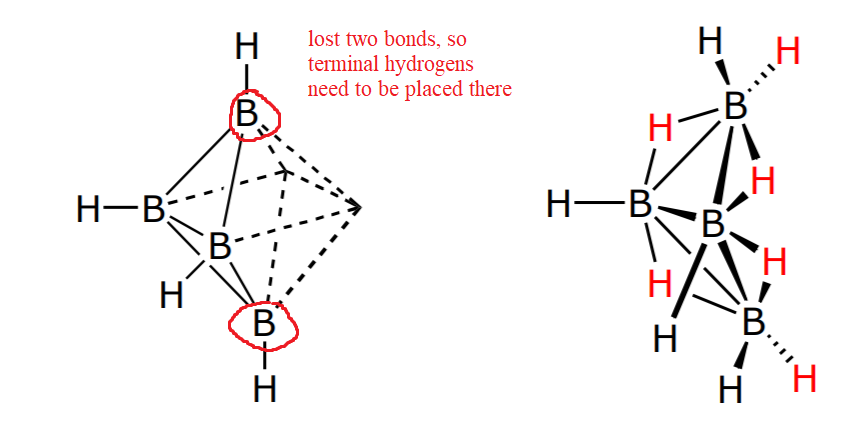
\includegraphics[width=10cm]{term.png}
    \end{figure}

    \newpage

    \subsubsection{Carboranes}
    Wade's rules also apply to carboranes, molecules where one or more of the Boron atoms have been replaces with a Carbon atom.
    The B-H and C-H\sup{+} fragments are said to be isolobal, meaning:
    \begin{itemize}
        \item They have the same number of electrons - isoelectronic.
        \item Their frontier orbitals (the HOMO and LUMO orbitals) have the same symmetries
        \item Their frontier orbitals are of similar energy
        \item Their frontier orbitals are of the same shape 
    \end{itemize}

    This means that the B-H and C-H units are interchangable in clusters and so we can use Wade's rules for them too. 

    Example C\sub{2}B\sub{3}H\sub{5}

    \begin{itemize}
        \item C\sub{2}B\sub{3}H\sub{5} = (CH)\sub{2}(BH)\sub{3} = (CH\sup{+})\sub{2}(BH)\sub{3} \sup{2}\sup{-} Since the C-H\sup{+} is positive we need a 2\sup{-} charge to be ditributed across the rest of the B-H units.
        \item Number of electrons, 6 (BH) + 4 (CH) + 2(BH negative charge) = 12 = 6 pairs, so n = 6
        \item n-1 = 5, 5 vertices so we have a trigonal bipyramid.
        \item CH + BH = 5 = n-1 so we have \textbf{CLOSO}
        \item However we have 3 different ways of arranging our CH units.
        \item The most stable form is having the two CH units be as far apart as possible, since they have CH\sup{+} units they will repell, so distance is stabibility.
        \item This means the most stable is the 1,5- structure 
    \end{itemize}

    \begin{figure}[h]
        \centering
        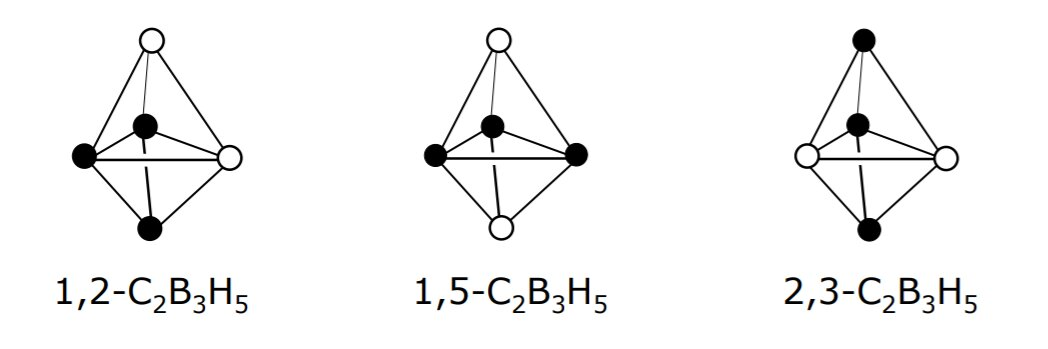
\includegraphics[width=10cm]{1-5.jpg}
    \end{figure}
    
    \subsection{The Tetrels}\thedate{Week 4}
    \\
    Group 14 elements, Carbon, Silicon, Germanium, Tin and Lead.
    \begin{itemize}
        \item Melting point lessens down the period
        \item Density greatens down the period
        \item Atomic radius greatens down the period
        \item Ionisation energy obviously lessens down the period
        \item Most common oxidation state is +4 except for Lead where it's +2
        \item Electronegativity lessens down the period  
        \item Oxides formed are normally \ce{MO_2} except for Lead which is most commonly \ce{PbO} and Carbon which can take both
        \item Carbon and silicone oxides are acidic (as expected from smaller more localised bonds) whilst the other oxides are amphoteric
        \item As expected when reacted with a Halogen you get \ce{MX_4} except for Lead which is \ce{MX_2}
    \end{itemize}
    \subsubsection{Hydrides}

    \ce{MH_4} is only formed up until Tin. We can see that the bond lengths get much larger down the period

    \begin{tabular}{l l}
        C-H & 1.09 \AA\\
        Si-H & 1.48 \AA\\
        Ge-H & 1.53 \AA\\
        Sn-H & 1.70 \AA
    \end{tabular}

    The M-H bonds get weaker down the group, a larger and more diffuse orbital, the bonds are a lot more polar and
    making it open to attack. Low lying LUMOS (easier for HOMO to be promoted?) also make it weaker.
    Because of this stability trend \ce{PbH_4} is so unstable no bond length has actually been measured.

    \subsubsection{Halides}
   
    \ce{CX_4} is very stable, however the rest of the tetrels are volatile and very susceptible to hydrolysis.
    \ce{SiCl_4 + 2H2O -> SiO2 + 4HCl}\\
    For \ce{Ge -> Pb} \ce{MX2} is also formed due to a more polar bond, lower lying LUMOs and a more electrophilic metalloid.

    \subsubsection{Silicone}

    Named after the apparent (but not actual) resemblence of \ce{Ph2SiO} to the Ketone \ce{Ph2CO}.
    They are nothing alike, \ce{Ph2SiO} is a polymer and they are not made the same.

    \begin{itemize}
        \item Hydrolysis of organohalides
        \item \ce{Me3SiCl + H2O -> Me3SiOH + HCl} This forms Silanol and HCl
        \item Under the presence of acid Silanol condeses
        \item \ce{2Me3SiOH ->[-H2O] Me3Si-O-SiMe3} siloxane, this does not happen with \ce{R3COH}
        \item To form polymeric siloxanes we need three types of monomers, the proportions of which will determine the properties of the siloxane polymer (silocone)
    \end{itemize}

    \begin{figure}[h]
        \centering
        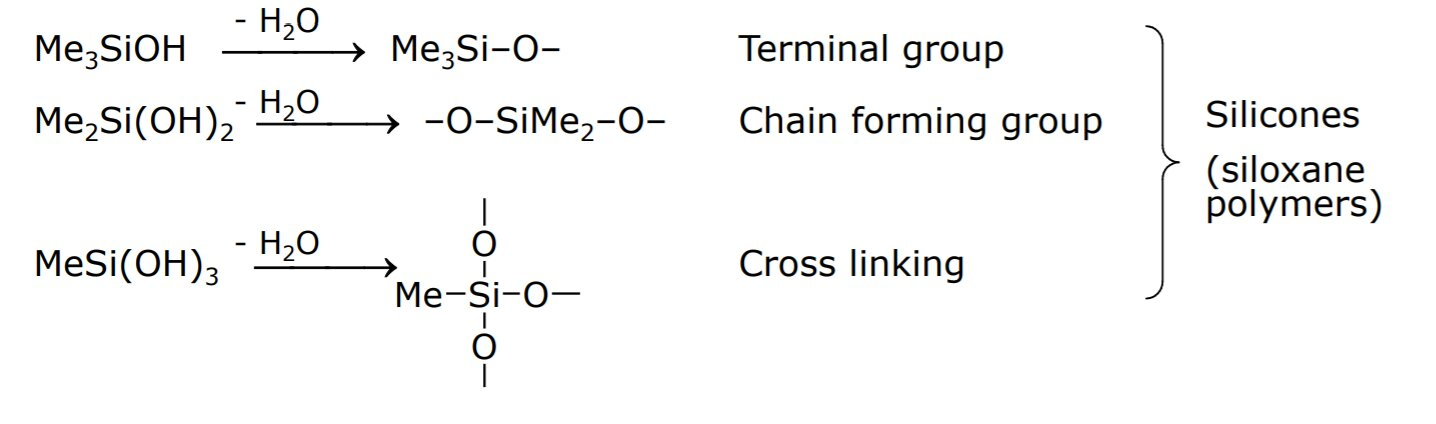
\includegraphics[width=10cm]{siloxanes.jpg}
    \end{figure}
    
    The thermal and chemical stability comes from the strengh of the Si-C bonds and the Si-O-Si bridges.

    Bond strengths $kJmol^{-1}$
    \begin{tabular}{l l l l l l}
        C-C & 346 & C-O & 357 & C-Si & 318\\
        Si-Si & 222 & Si-O & 452 & Si-Cl & 381
    \end{tabular}

    Very invert but will react with fluorinating ages, \ce{Si-F} is very strong, also with concentrated \ce{OH} solutions.
    The \ce{Si-O} bond is very strong because of the back bonding from oxygen to empty silicon.
    
    \begin{figure}[h]
        \centering
        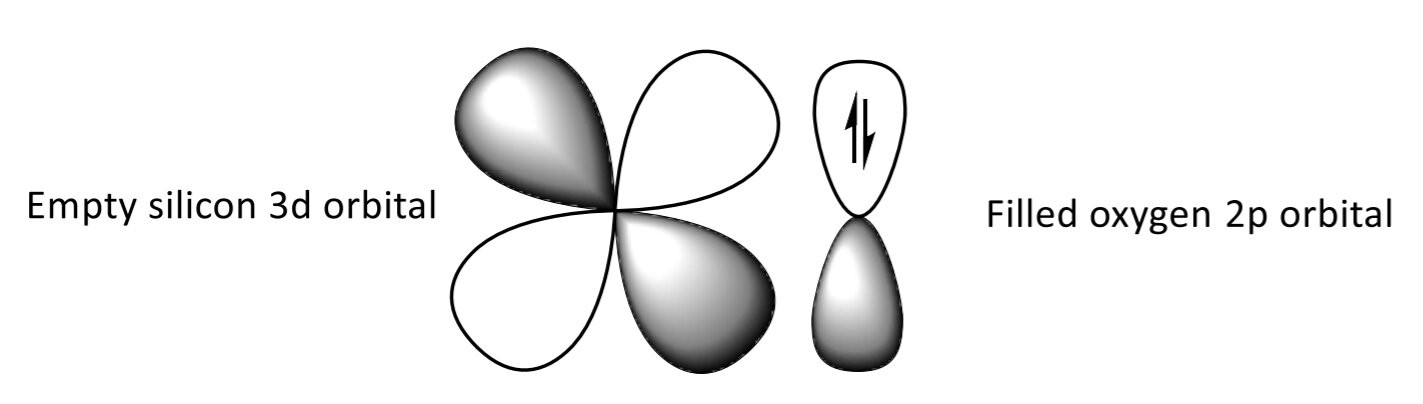
\includegraphics[width=10cm]{backbon.jpg}
    \end{figure}

    It's easy to make double and triple bonds with first row elements because of the good orbital overlap, 
    whilst it is possible to make $\pi$ bonds with the heavier group 14 elements $\sigma$ bonds will always be prefered.

     \subsubsection{Zintl ions (with Wade's Rules)}

    The reductions of Lead with Soidum formed these ions. \ce{Pb ->[Na][NH3] 4Na+ + [Pb9]^{4-}}
    The use of cryptand ligands enables the crystallisation of these compounds
    \ce{[Pb0]^{4-} + Pb ->[crypt-222][NH3] 2[Pb5]^{2-}}

    Zintl ions can contain group 1 and 2 metals along with the post transition group 12 metals, or mettaloids from 13 to 16

    \begin{figure}[h]
        \centering
        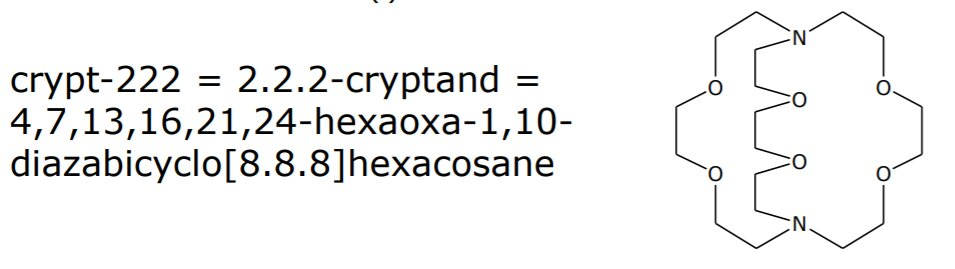
\includegraphics[width=10cm]{crypt.jpg}
    \end{figure}

    The Sodium ion is bound inside this compound, meaning it can't pair with the lead cluster

    \subsection{The Pnictogens}
    Assessing trends down group 15
    \begin{itemize}
        \item Ionisation energy goes down
        \item Electron affinity goes up
        \item Electronegativity goes down
        \item Nitrogen takes oxidation states -3, +1 to +5, P and As +3 and +5, and Sb and Bi only take +3
        \item Atomic radius goes up
    \end{itemize}

    Nitrogen triple bond is the most stable bond possible so the forming of it is very favourable, this makes 
    \ce{N2} a common end product in explosives. The \ce{N^{3-}} ion does exist. \ce{6Li + N2 -> 2Li3N}, \ce{Li+}
    is very small and so the lattice energy is very high. There is very little catenation (joing of atoms, like in benzene)
    due to a weak N-N bond.\\

    Phosphorous has many alletropes because of catenation. White, black and red phosphorous. 
    Red phosphorous has a layered structured, similar to those that As, Sb and Bi form. The elements become
    more metallic down the group.\\

    Phosprous forms P(III) and P(V) oxides, \ce{P4O6} and \ce{P4O10}. Whilst Nitrogen forms 7 oxides, all of which
    are less stable than \ce{N2} and \ce{O2}\\

    They all form Hydrides of \ce{EH3}, the bond energy decreases down the group and so the stability decreases.
    \begin{figure}[h]
        \begin{tabular}{l l l l}
            N & P & As & Sb\\
            106.7 & 93.6 & 92.1 & 91.6
        \end{tabular}
        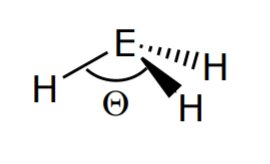
\includegraphics[width=5cm]{eh3.jpg}
    \end{figure}

    \ce{NH3} has a relatively high boiling point (-33$^\circ$C), hight polarity and H bonding. \ce{NH3} (ammonia) is basic.
    \ce{PH3} is not basic, as the P-H bonds are p$\sigma$-s$\sigma$ and the 3s orbital in P contributes little to the bonding, it is the lone pair.

    \begin{figure}[h]
        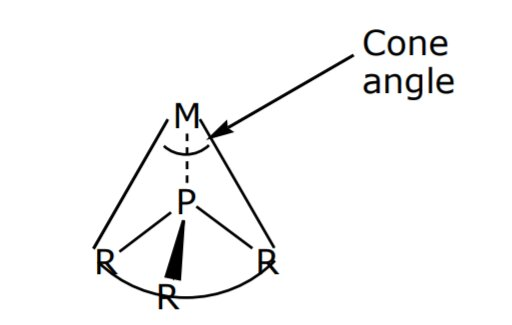
\includegraphics[width=5cm]{cone.jpg}
    \end{figure}

    When bonding to a metal, \ce{PR3} is a goodl ligand, the cone angle increases for bigger R groups, this affects
    other ligands which are attached to the metal. \\

    For the \ce{MX3} halides all of them are formed, but for \ce{MX5} this is not the case

    \begin{tabular}{l l l l l}
         & F & Cl & Br & I\\
      P  & Y  & Y & Y & Y \\
      As & Y & Y & N & N\\
      Sb & Y & Y & N & N\\
      Bi & Y & N & N & N
    \end{tabular}

    \ce{NF3} has a boiling point os -129, bond angle of 102, which is less than \ce{NH3} which is 107.
    In \ce{PF3} the electronegativity of F lowers the energy of the P 3d orbitals and so it has good $\pi$ backbonding.
    In the solid state \ce{PCl5} exists as tetrahedral \ce{[PCl4]+} and Octehedral \ce{[PCl6]-}, but in the gaseous phase
    it's just regular trigonal bipyramidal. In \ce{PBr5} a \ce{Br-} anion dissociates and so it takes the form \ce{[PBr4]+Br-}.
\end{document}